
\let\negmedspace\undefined
\let\negthickspace\undefined
\documentclass[journal,12pt,twocolumn]{IEEEtran}
\usepackage{cite}
\usepackage{amsmath,amssymb,amsfonts,amsthm}
\usepackage{algorithmic}
\usepackage{graphicx}
\usepackage{textcomp}
\usepackage{xcolor}
\usepackage{txfonts}
\usepackage{listings}
\usepackage{enumitem}
\usepackage{mathtools}
\usepackage{gensymb}
\usepackage[breaklinks=true]{hyperref}
\usepackage{tkz-euclide} % loads  TikZ and tkz-base
\usepackage{listings}
\usepackage{gvv}
\usepackage{floatrow}
%
%\usepackage{setspace}
%\usepackage{gensymb}
%\doublespacing
%\singlespacing

%\usepackage{graphicx}
%\usepackage{amssymb}
%\usepackage{relsize}
%\usepackage[cmex10]{amsmath}
%\usepackage{amsthm}
%\interdisplaylinepenalty=2500
%\savesymbol{iint}
%\usepackage{txfonts}
%\restoresymbol{TXF}{iint}
%\usepackage{wasysym}
%\usepackage{amsthm}
%\usepackage{iithtlc}
%\usepackage{mathrsfs}
%\usepackage{txfonts}
%\usepackage{stfloats}
%\usepackage{bm}
%\usepackage{cite}
%\usepackage{cases}
%\usepackage{subfig}
%\usepackage{xtab}
%\usepackage{longtable}
%\usepackage{multirow}
%\usepackage{algorithm}
%\usepackage{algpseudocode}
%\usepackage{enumitem}
%\usepackage{mathtools}
%\usepackage{tikz}
%\usepackage{circuitikz}
%\usepackage{verbatim}
%\usepackage{tfrupee}
%\usepackage{stmaryrd}
%\usetkzobj{all}
%    \usepackage{color}                                            %%
%    \usepackage{array}                                            %%
%    \usepackage{longtable}                                        %%
%    \usepackage{calc}                                             %%
%    \usepackage{multirow}                                         %%
%    \usepackage{hhline}                                           %%
%    \usepackage{ifthen}                                           %%
  %optionally (for landscape tables embedded in another document): %%
%    \usepackage{lscape}     
%\usepackage{multicol}
%\usepackage{chngcntr}
%\usepackage{enumerate}

%\usepackage{wasysym}
%\documentclass[conference]{IEEEtran}
%\IEEEoverridecommandlockouts
% The preceding line is only needed to identify funding in the first footnote. If that is unneeded, please comment it out.

\newtheorem{theorem}{Theorem}[section]
\newtheorem{problem}{Problem}
\newtheorem{proposition}{Proposition}[section]
\newtheorem{lemma}{Lemma}[section]
\newtheorem{corollary}[theorem]{Corollary}
\newtheorem{example}{Example}[section]
\newtheorem{definition}[problem]{Definition}
%\newtheorem{thm}{Theorem}[section] 
%\newtheorem{defn}[thm]{Definition}
%\newtheorem{algorithm}{Algorithm}[section]
%\newtheorem{cor}{Corollary}
\newcommand{\BEQA}{\begin{eqnarray}}
\newcommand{\EEQA}{\end{eqnarray}}
\newcommand{\define}{\stackrel{\triangle}{=}}
\theoremstyle{remark}
\newtheorem{rem}{Remark}

%\bibliographystyle{ieeetr}
\begin{document}

\bibliographystyle{IEEEtran}


\vspace{3cm}

\title{
ASSIGNMENT-1
}
\author{ KUNWAR DUSHYANT SINGH EE22BTECH11031}


\maketitle

\newpage

%\tableofcontents

\bigskip

\renewcommand{\thefigure}{\theenumi}
\renewcommand{\thetable}{\theenumi}

Question 1.3.3 

$D_{1}$ is a point on $\vec{B}$$\vec{C}$ such that
$\vec{A}$$\vec{D_{1}}$$\perp$ $\vec{B}$$\vec{C}$ and $\vec{A}$$\vec{D_{1}}$  is defined to be the altitude.
Find the equations of the altitude $\vec{B}$$\vec{E_{1}}$ and $\vec{C}$$\vec{F_{1}}$
to the sides $\vec{A}$$\vec{C}$ and $\vec{A}$$\vec{B}$ respectively.
\\ \solution
Given:
\begin{align}\vec{A}=\myvec{1\\-1} \\
\vec{B}=\myvec{-4 \\6} \\
\vec{C}=\myvec{-3\\-5}
\end{align}
Direction vector 
\begin{align}
\vec{m}_{AB}&=\vec{B}-\vec{A} \\
&=\myvec{-4\\6}-\myvec{1\\-1} \\
&=\myvec{-5\\7} \\
\vec{m}_{AC}&=\vec{C}-\vec{A} \\
&=\myvec{-3\\-5\\}-\myvec{1\\-1} \\
&=\myvec{-4\\-4\\}
\end{align}
Normal vector of $BE_{1}$ is orthogonal to $BE_{1}$ and hence parallel to $AC$ and normal vector of $CF_{1}$ is orthogonal to $CF_{1}$ and hence parallel to $AB$ 
\begin{align}
\vec{n}_{BE_{1}}&=\vec{m}_{AC} \\
&=\myvec{-5\\7} \\
\vec{n}_{CF_{1}}&=\vec{m}_{AB} \\
&=\myvec{-4\\-4}
\end{align}
Equation of line is represented by:
\begin{align}
\vec{n}^{\top}(\vec{x}-\vec{p})=0
\end{align}
\begin{enumerate}
\item The equation of line $\vec{C}$$\vec{F_{1}} $
\begin{align}
\vec{n}_{CF_{1}}^{\top}\brak{\vec{x}-\vec{C}}&=0 \\
\myvec{-5 \\7}^\top\brak{\vec{x}-\myvec{-3\\-5}}&=0 \\
\myvec{-5 & 7}\brak{\vec{x}-\myvec{-3\\-5}}&=0  \\
\myvec{-5\\7}^\top\vec{x}=-20
\end{align}
\item The equation of line $\vec{B}$$\vec{E_{1}}$ 
\end{enumerate}
\begin{align}
\vec{n}_{BE_{1}}^{\top}\brak{\vec{x}-\vec{B}}&=0 \\
\myvec{-4 \\-4}^\top\brak{\vec{x}-\myvec{-4\\6}}&=0 \\
\myvec{-4&-4}\brak{\vec{x}-\myvec{-4\\6}}&=0  \\
\myvec{-4\\-4}^\top\vec{x}&=-8
\end{align}
\begin{figure}[H]
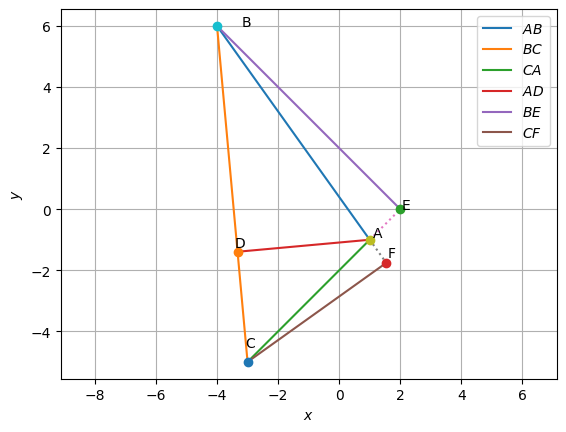
\includegraphics[width=\columnwidth]{figs/main.png}
\caption{Lines $\vec{BE}_{1}$ and $\vec{CF}_{1}$ }
\label{fig:i_tri_py}
\end{figure}
\end{document}

